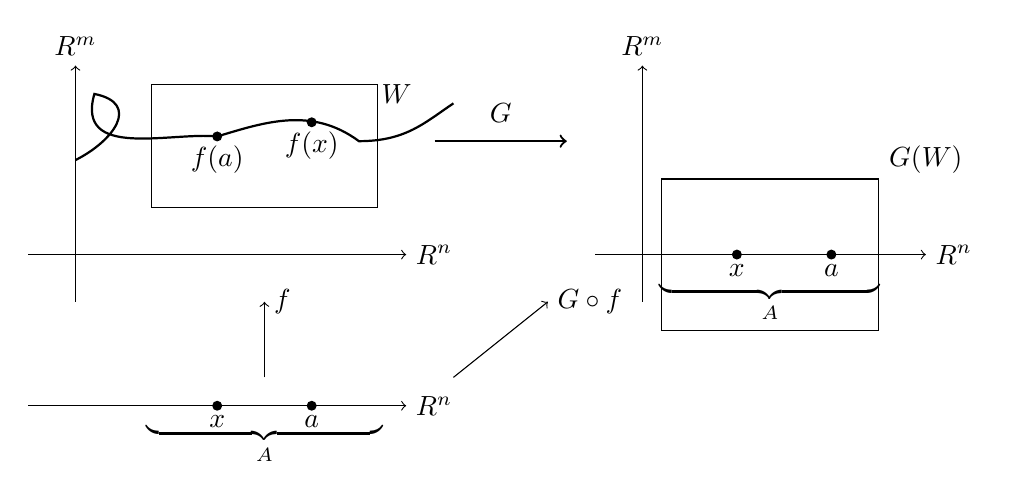
\begin{tikzpicture}[scale=1.2]

  % Ejes izquierda
  \draw[->] (-3,-0.5) -- (-3,2) node[above] {$\mathbb{R}^m$};
  \draw[->] (-3.5,0) -- (0.5,0) node[right] {$\mathbb{R}^n$};

  % Puntos en A
  \fill (-0.5,1.4) circle (1.5pt) node[below] {$f(x)$};
  \fill (-1.5,1.25) circle (1.5pt) node[below] {$f(a)$};
  
  % Rectángulo (W)
  \draw (-2.2,0.5) rectangle (0.2,1.8);
  \node at (0.4,1.7) {$W$};
  
  % Curva dentro
      \draw[thick] 
      (-3,1) 
      .. controls (-2.6,1.2) and (-2.3,1.6) .. (-2.8,1.7)
      .. controls (-3,1) and (-2,1.3) .. (-1.5,1.25)
      .. controls (-1,1.4) and (-0.5,1.57) .. (0,1.2)
      .. controls (0.5,1.2) and (0.7,1.4) .. (1,1.6);
  
  % Flecha F
  \draw[->, thick] (0.8,1.2) to[out=0,in=180] (2.2,1.2);
  \node at (1.5,1.5) {$G$};
  
  % Ejes derecha
  \draw[->] (3,-0.5) -- (3,2) node[above] {$\mathbb{R}^m$};
  \draw[->] (2.5,0) -- (6,0) node[right] {$\mathbb{R}^n$};
  
  
  % Rectángulo G(W)
  \draw (3.2,-0.8) rectangle (5.5,0.8);
  \node at (6,1) {$G(W)$};
  
  % Conjunto A (intervalo)
  \draw (-2,0) -- (0,0);
  \node at (4.35,-0.5) {
      $\underbrace{\hspace{2.8cm}}_{A}$
  };
  
  % Puntos imagen
  \fill (4,0) circle (1.5pt) node[below] {$x$};
  \fill (5,0) circle (1.5pt) node[below] {$a$};
  
  % Flecha hacia abajo (A a c)
  \draw[->] (-1,-1.3) -- (-1,-0.5) node[right] {$f$};
  \draw[->] (1,-1.3) -- (2,-0.5) node[right] {$G\circ f$};
  
  % Línea inferior
  \fill (-1.5,-1.6) circle (1.5pt) node[below] {$x$};
  \fill (-0.5,-1.6) circle (1.5pt) node[below] {$a$};
  \draw[->] (-3.5,-1.6) -- (0.5,-1.6) node[right] {$\mathbb{R}^n$};

  % Conjunto A (intervalo)
  \draw (-2,0) -- (0,0);
  \node at (-1,-2) {
    $\underbrace{\hspace{3cm}}_{A}$
  };

\end{tikzpicture}
